\chapter{Mérési eredmények}
%%%%%%%%%%%%%%%%%%%%%%%%%%%%%%%%%%%%%%%%%%%%%%%%%
%(12-15 oldal)



%\section{Mérési eredmények}
%(7-10 oldal): kinyert mérések tartalma(delay, jitter, link, AS info, Geolocation), mérések mennyisége, mérések minősége

\section{Létrehozott adatbázis bemutatása}
Jelen fejezet bemutatja a létrehozott adatbázis fontosabb adathalmazait, amelyek további elemzések alapját képezi.

\subsection*{Éllista}
A legfontosabb eredmény az internetes útvonalakat alkotó gépek közötti kapcsolatokról szolgáltat mérési eredményeket. Az objektum amelyről a mérés készült egy internetes link, a kinyert információk a következők:

\begin{itemize}
\item \textbf{delay:} késleltetés a két gép közötti kapcsolaton
\item \textbf{rtt:} A from számítógéphez végzett körülfordulási idő a mérést végző measurer\_ip számítógéptől
\item \textbf{time:} A mérés időpontja
\item \textbf{jitter:} Késleltetés ingadozás a két számítógép között
\item \textbf{measurer\_ip:} A mérést végző számítógép (ahol a traceroute parancs fut)
\item \textbf{target\_ip:} Az útvonalmérés célpontja
\item \textbf{to:} A mérést végző számítógéptől távolabbi csomópont információi: city, country, longitude, latitude, ip, asn
\item \textbf{from:} A mérést végző számítógéphez közelebbi csomópont információi: city, country, longitude, latitude, ip, asn
\end{itemize}

\subsection*{PlanetLab gépek állapota}
A PlanetLab gépek eléréséről (az operációs rendszeréről) és hiba esetén a hibaüzenetek aggregált statisztikája. A következő adatokat tartalmazza:

\begin{itemize}
\item \textbf{erroneous:} Sikertelen csatlakozások száma (online gépek esetén)
\item \textbf{succeed:} Gépek száma, amelyeken sikeres volt a távoli parancsfuttatás (cat /etc/issue)
\item \textbf{online:} A ping parancssal elérhető gépek száma
\item \textbf{offline:} A ping parancssal nem elérhető gépek száma
\item \textbf{outputs:} Az összes különböző kimenet felsorolása a hozzá tartozó előfordulások számával.
\item \textbf{error\_types:} Az összes különböző hibatípus felsorolása a hozzá tartozó előfordulások számával
\item \textbf{ts:} A mérés időpontja
\end{itemize}

\subsection*{AS gráf él információi}
A korábban részletesen bemutatott AS gráf ezen kollekció adataiból lett felépítve:

\begin{itemize}
\item \textbf{asn:} A autonóm rendszer azonosító száma
\item \textbf{core\_ips:} Az autonóm rendszeren belül észlelt ip címek
\item \textbf{gateways\_to\_as:} Az autonóm rendszerből másikba vezető kapcsolatok listája. A másik AS-hez irányuló ip cím párok (egyik AS kimeneti címe, másik AS bemeneti címe) listáit is tartalmazza.
\end{itemize}



\begin{figure}[h]
	\centering
	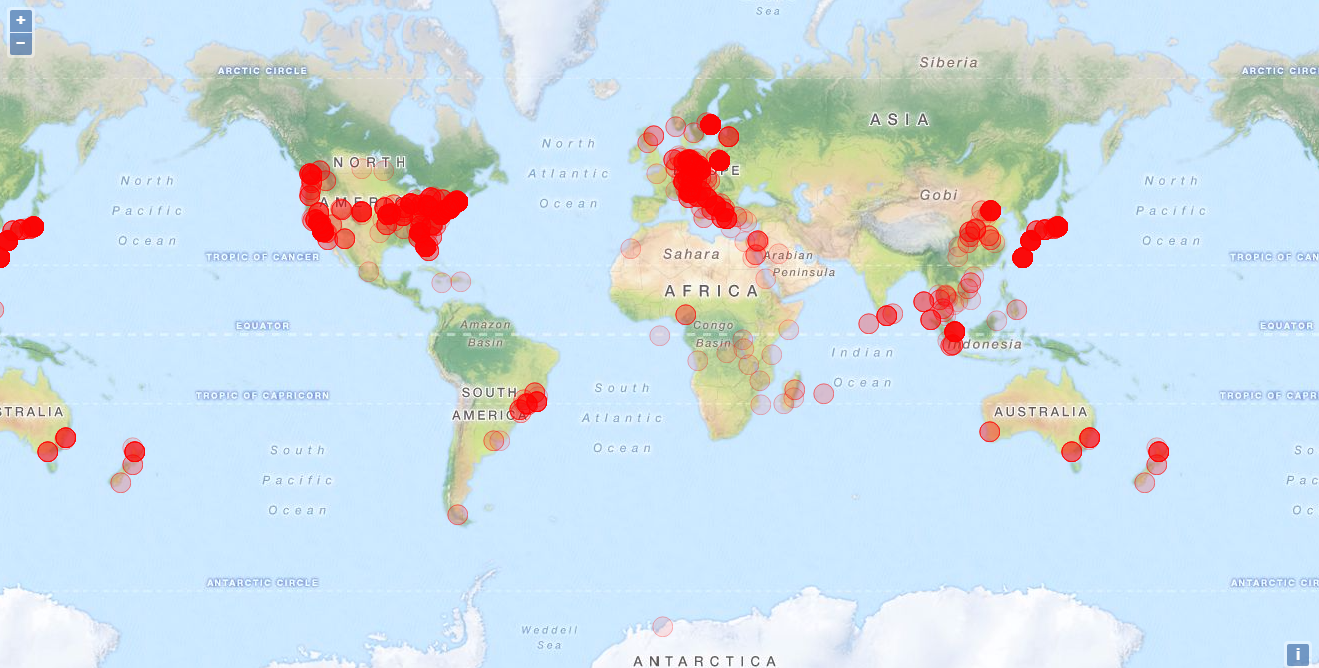
\includegraphics[width=0.9\textwidth, keepaspectratio]{figures/ip_map.png}
	\caption{A mérésben résztvevő ip címek geolokációs pozíciójai}
	\label{fig:ip-map}
\end{figure}

\section{Gráf ábrázolása}

Az gráf tulajdonságainak intuitív leolvasásához ábrázolások készültek. Mivel már egy mérés során több mint 1700 csomópontból álló gráfot kell ábrázolni, ezért ennek kivitelesése nehézségekbe ütközik. A \ref{fig:graph} ábrán látható egy ilyen gráf leképezés.

\begin{figure}[!ht]
	\centering
	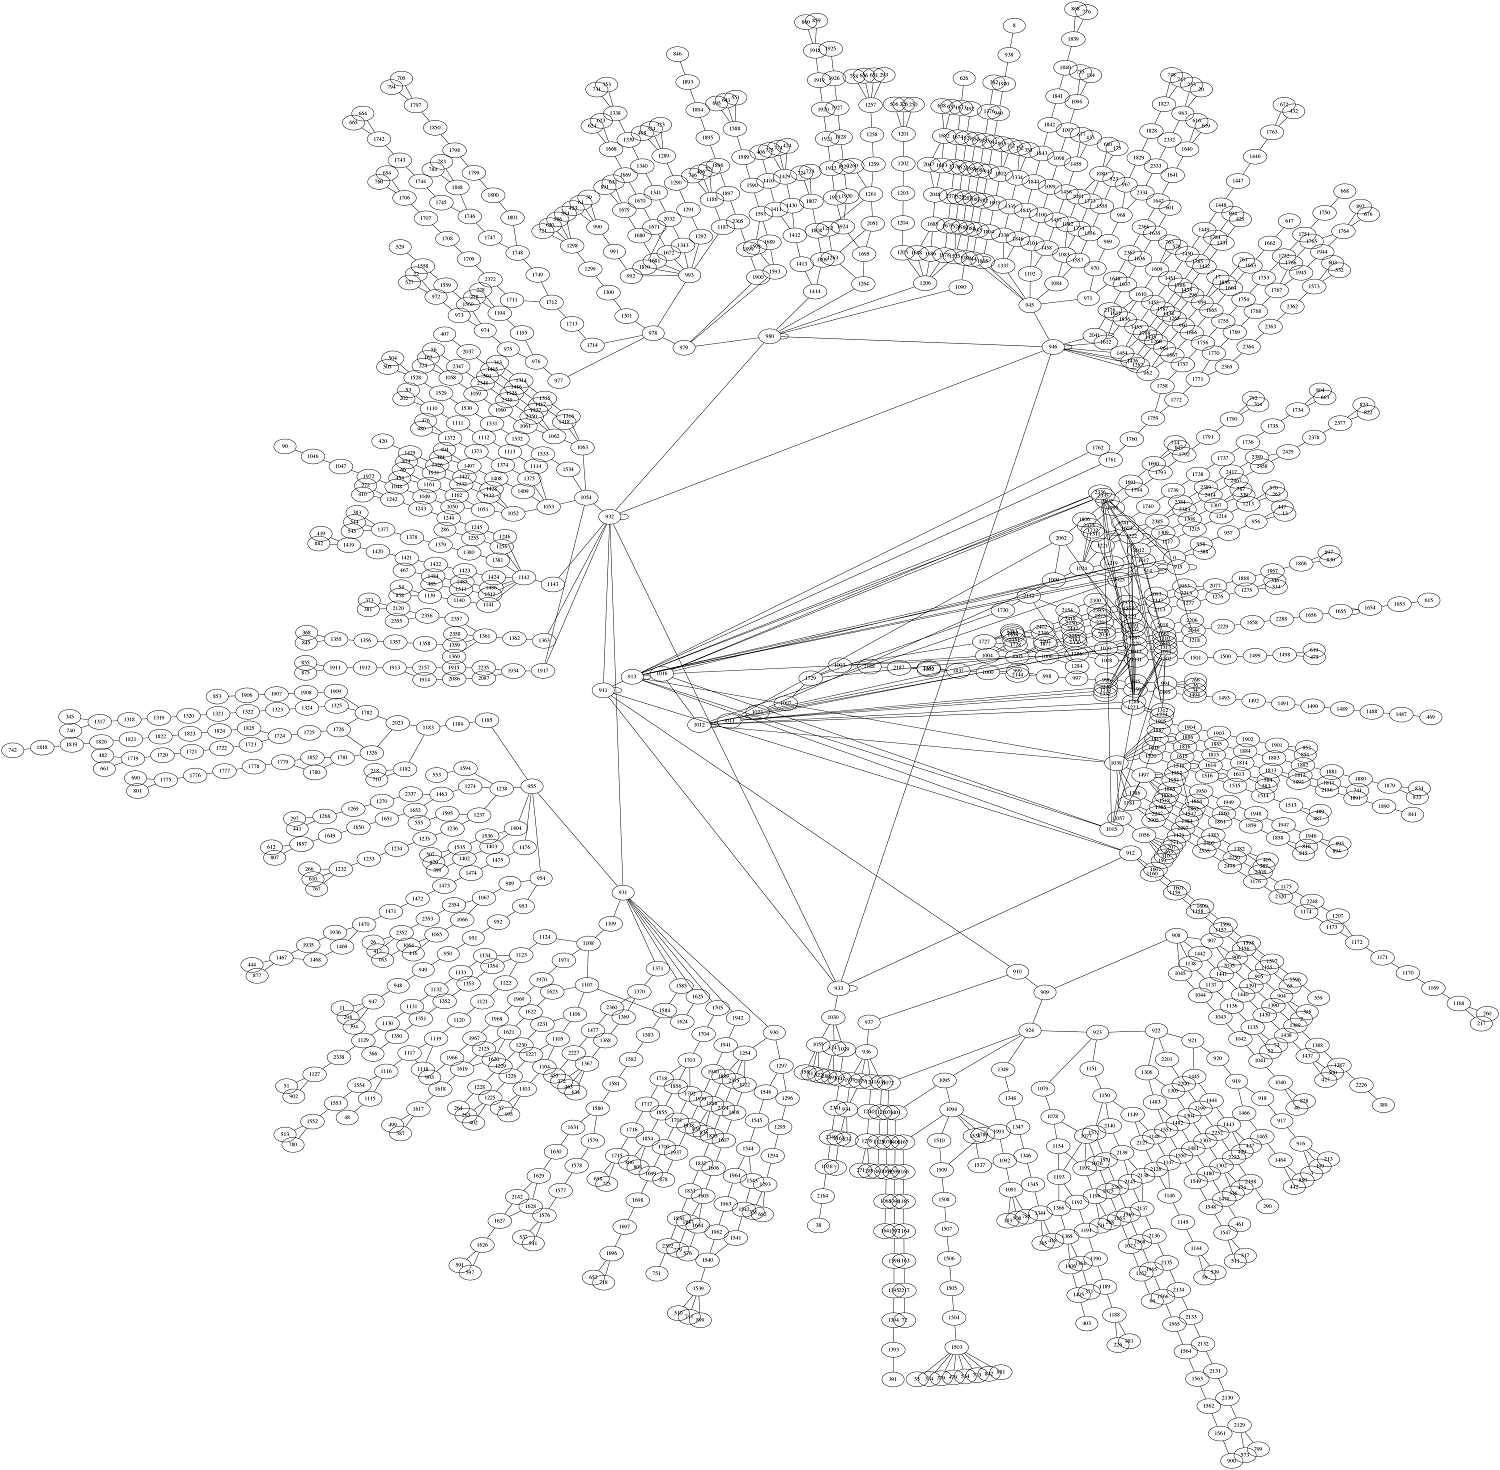
\includegraphics[width=1\textwidth, keepaspectratio]{figures/graph.png}
	\caption{Egy napi mérés gráfja csak az egyik IP címhez menő útvonalakból\label{fig:graph}}
\end{figure}

Az ezen a képen jól láthatóak a középponttól távolodó hosszú fürtök, melyek egy cél IP cím AS-éhez vezető többnyire független útvonalakat reprezentálja.

\begin{figure}[h]
	\centering
	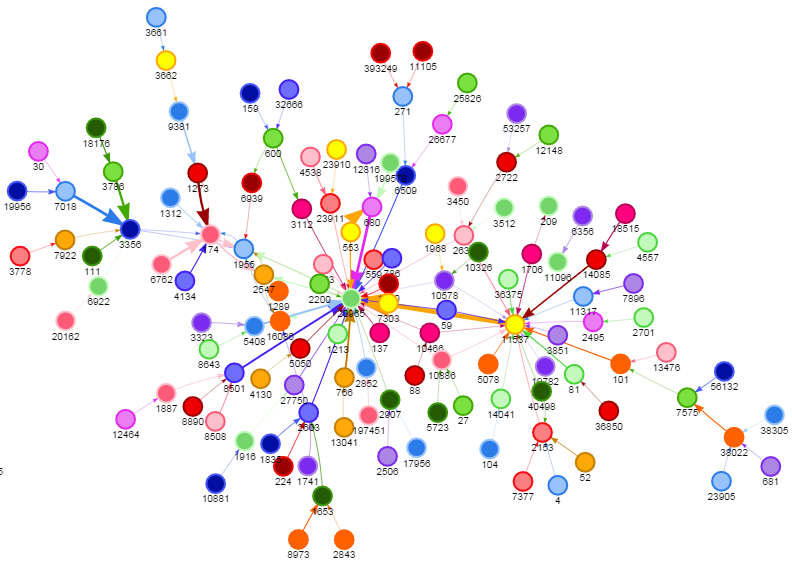
\includegraphics[width=0.95\textwidth, keepaspectratio]{figures/as-graph.png}
	\caption{A PlanetLab gépeitől az egyetem felé küldött csomagok által bejárt AS gráf}
	\label{fig:as-graph}
\end{figure}

Az AS szám információ felhasználásával a \ref{fig:as-graph} ábrán látható gráf lett elkészítve. Az ábra adatforrása pár nap folyamatos traceroute mérések eredménye. A PlanetLab csatlakozott gépeiről a BME egyik gépe felé címzett útvonalak lettek aggregálva. A nyilak vastagsága az alapján növekszik, hány különböző ip cím pár köti össze a két AS csomópontot. Ha minden átmenő csomag azonos ip címeken halad keresztül akkor az vékony lesz, míg ha két AS között haladó csomagok több különböző ip cím párokon keresztül utaznak az vastagabban van ábrázolva.

A \ref{fig:as-graph} ábráról leolvasható hogy mely AS-ek kiterjedtek geolokációs tekintetben. Ha ugyanis több különböző ip útvonal köt össze két AS-t akkor azok valószínűleg területileg is több ponton vannak összeköttetésben.

A \ref{fig:as-graph} ábrán az összes útvonal a BME AS2547-es csomópontjába irányul, amely a valóságban kizárólag a AS1955-ös HBONE-AS HUNGARNET-tel van összeköttetésben. Egyes hibás traceroute mérések azonban torzítják ezt. A legnagyobb fokszámú csomópont az AS20965 , amely az AS1955 legfontosabb szomszédja, az elvi 17-ből\footnote{Forrás: Európai Regionális Internetes Nyilvántartó Hivatal honlapja: \href{https://stat.ripe.net/widget/asn-neighbours\#w.resource=1955}{stat.ripe.net}}.